In this section we describe our methodology, 
briefly describing the datasets and features computed, as well as the model
architectures and GAN algorithms used.
\subsection{Datasets}
In our experiments, we use the MNIST dataset, a MIDI dataset of 389 Bach
Chorales downloaded from the web and a subsample of the NIST 2004 telephone
conversational speech dataset with 100 speakers, multiple languages and
on average 5 minutes of audio per speaker.

\subsection{Property extraction}
The properties extracted from the datasets used on this paper can be
perceptually meaningful or not. We claim that both properties can be used to numerically identify the source of the sample. In the context of this
paper, samples are images of size 64 by 64. 

\subsubsection{Spectral Moments}
The spectral centroid~\cite{peeters2004large} is a feature commonly used in the
audio domain, where it represents the barycenter of the spectrum. This feature
can be applied to other domains and we invite the reader to visualize 
Figure~\ref{fig:centroids} for examples on MNIST and
Mel-Spectrograms~\cite{peeters2004large}. For each column in an image, we 
transform the pixel values into row probabilities by normalizing them by the
column sum, after which we take the expected row value, thus obtaining the
spectral centroid.

Figure~\ref{fig:mnist_centroids} shows the spectral centroid computed
on sample of MNIST training data.

\begin{figure}[!h]
    \centering
    \begin{subfigure}[b]{0.4\textwidth}
        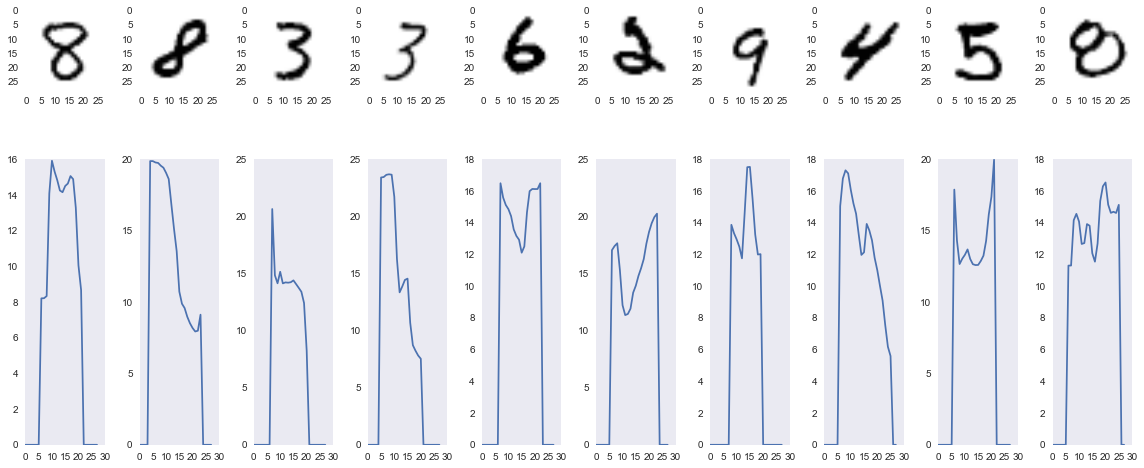
\includegraphics[width=\linewidth]{mnist_centroids.png}
        \caption{MNIST samples and centroids}
        \label{fig:mnist_centroids}
    \end{subfigure}
    \quad
    \begin{subfigure}[b]{0.4\textwidth}
        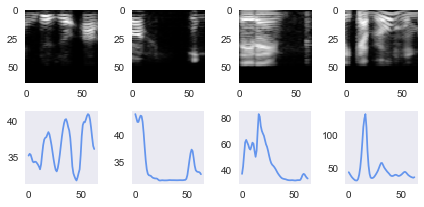
\includegraphics[width=\linewidth]{speech_spectral_centroids.png}
        \caption{Mel-Spectrograms and centroids}
        \label{fig:spectrogram_centroids}
    \end{subfigure}
    \caption{Spectral centroids on digits and Mel-Spectrograms}
    \label{fig:centroids}
\end{figure}

\subsubsection{Spectral Slope}
The spectral slope adapted from~\cite{peeters2004large} is computed by applying linear regression using an overlapping
sliding window of size 7. For each window, we regress the spectral centroids on
the column number \textit{mod} the window size. Figure~\ref{fig:slopes} shows these
features computed on MNIST and Mel-Spectrograms. 

\begin{figure}[!h]
    \centering
    \begin{subfigure}[b]{0.4\textwidth}
        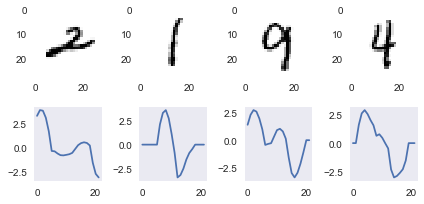
\includegraphics[width=\linewidth]{mnist_slopes.png}
        \caption{MNIST samples and slopes}
        \label{fig:mnist_slopes}
    \end{subfigure}
    \quad
    \begin{subfigure}[b]{0.4\textwidth}
        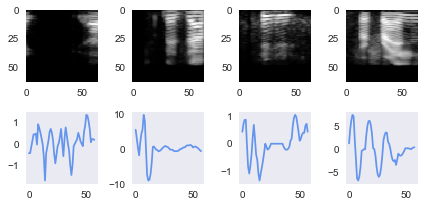
\includegraphics[width=\linewidth]{speech_spectral_slopes.png}
        \caption{Mel-Spectrograms and slopes}
        \label{fig:spectrogram_slopes}
    \end{subfigure}
    \caption{Spectral slopes on digits and Mel-Spectrograms}
    \label{fig:slopes}
\end{figure}

\subsection{Generative Models}
We investigate samples produced with the DCGAN architecture using the
Least-Squares GAN (LSGAN)~\cite{mao2016least} and the improved Wasserstein
GAN (IWGAN)~\cite{gulrajani2017improved}. We also compare adversarial MNIST
samples produced with the fast gradient sign method
(FGSM)~\cite{goodfellow2014explaining}.
